\documentclass{article}
\usepackage[utf8]{inputenc}
\usepackage{algorithm}
\usepackage{algorithmic}
\usepackage{amsfonts}
\usepackage{graphicx}
\usepackage{listings}
\usepackage{xcolor}
\usepackage{amsmath}
\usepackage{amsthm,amssymb}
\theoremstyle{definition}
\theoremstyle{theorem}
\usepackage{geometry}
\geometry{a4paper,left=25mm,right=25mm,bottom=25mm,top=25mm,footskip=15mm}
\newtheorem{definition}{Definíció}
\newtheorem{theorem}{Tétel}

\newtheorem{example}{Példa}
\renewcommand{\qedsymbol}{\rule{0.7em}{0.7em}}
\title{Szakdolgozat}
\author{Szabó Bence Dániel }
\date{Date}

\definecolor{codegreen}{rgb}{0,0.6,0}
\definecolor{codegray}{rgb}{0.5,0.5,0.5}
\definecolor{codepurple}{rgb}{0.58,0,0.82}
\definecolor{backcolour}{rgb}{0.95,0.95,0.92}

\lstdefinestyle{mystyle}{
    backgroundcolor=\color{backcolour},
    commentstyle=\color{codegreen},
    keywordstyle=\color{magenta},
    numberstyle=\tiny\color{codegray},
    stringstyle=\color{codepurple},
    basicstyle=\ttfamily\footnotesize,
    breakatwhitespace=false,
    breaklines=true,
    captionpos=b,
    keepspaces=true,
    numbers=left,
    numbersep=5pt,
    showspaces=false,
    showstringspaces=false,
    showtabs=false,
    tabsize=2
}
\lstset{style=mystyle}
\begin{document}

\begin{center}
\fontsize{40pt}{12pt}\selectfont

    DIFFERENCIÁLEGYENLETEK NUMERIKUS MEGKÖZELÍTÉSE A KÖZGAZDASÁGBAN\\
    \bigskip
    Témavezető: Kánnai Zoltán\\
    \bigskip
    Készítette: Szabó Bence Dániel\\
    \bigskip
    Szak : Gazdaság-és pénzügy matematikai elemzés
\end{center}

\pagebreak
\tableofcontents
\pagebreak
\section{Bevezetés}
A szakdolgozatom fő célkitűzése az, hogy körbejárjam néhány differenciál egyenlet típus numerikus megoldásainak egy részét. Legfőképp kezdetiérték feladatokról lesz szó a témák körbejárása alatt. A numerikus részt pedig úgy próbálom teljesíteni, hogy ahol tudtam, ott az elmélet mellé csatoltam kódot is. A kódokat Pythonban írtam meg és ahol vannak számítási eredmények, ott ezekből a kódokból érkeznek a szakdolgozatba. Amikor csatoltam egy kódot azt próbáltam minnél olvashatóbban tagolni, például követve a flake8 csomag útmutatásait a formázásra nézve. Az volt az elgondolásom, hogy úgy lesz kerek és egész a dolgozat, ha az eszközökről is teszek említést, amivel írtam a munkát, ezért pedig egy rövid Python leírást is készítettem, abban pedig megemlítem a használt csomagokat. Ezen felül egy úgyszintén tömör összefoglalót is mellékeltem a nyelv felépítéséről, működéséről . A differenciál egyenletek témaköre amiatt keltette fel az érdeklődésemet, mert mindig is érdekelt a programozás és ehhez a témakörhöz sok numerikus kutatás készült már, amelyek szépen programozhatóak. Mind a közgazdasági, mind pedig pénzügyi modellek között vannak differenciálegyenletek. Az előbbi inkább nem sztochasztikus, az utóbbi inkább sztochasztikus modellekre épít. A sztochasztikus modellek mögötti matematika egy lépcsőfokkal bonyolultabb a nem sztochasztikus egyenleteknél, a szakdolgozatom is inkább erre a témára helyezi a hangsúlyt.
\section{Szakirodalmi áttekintő}
A differenciál egyenletek használata nagyon sok területen megjelenik a matematikán belül. Az egyik leginkább elterjedt ága ennek a tudománynak a dinamikai rendszerek alkalmazása közgazdasági modellekre. Itt alapvetően azt vizsgálják a kutatók, hogy az idő változásával hogyan és miképp változik meg egy - egy rendszer és annak a változói. Amint feltudtuk írni az egyenleteket akkor vizsgálhatjuk a rendszer stabilitáselméleti 'diagnosztikáit', amit majd látjuk a következő részekben, hogy a sajátértékek vizsgálatából von le következtetéseket, amit felhasználva tudunk valamit mondani a renszer időbeli fejlődéséről. Ilyen lehet például egy ország adósságrátája vagy a GDP - je. A. Tacchella et. al (2018) egy olyan dinamikai rendszert építettek, amely a vizsgált országok GDP változását (akár növekedését, akár csökkenésést) volt hivatott előrejelezni. A szerzők megemlítik, hogy a GDP előrejelzés egy nehéz és komplex feladat, mivel rengeteg változóból épül fel ez a negyedévente / évente megszülető adat, ezen feül sok utólagos korrigálásban részesülnek az adatok, amelyek nem jól modellezhetőek, mert szubjektívan készítik el őket. Az eredményeiket jelentősnek írták le, mivel 25 százalék feletti eredménnyel jelezték előre a változást a hivatalos IMF statisztikákhoz képest, ezenfelül az IMF hibái és ő hibáik között alacsony volt a korreláció, ami azt jelenti, hogy az eltéréseik között nem volt érdemi információs átfedés, így új összefüggésekre tudtak rámutatni. A szerzők kiemelnek egy fontos tényezőt a közgazdasági modellezéssel kapcsolban, hogy maga a közgazdaságtan, az elméleti modellezés és az előrejelzés tudomány ágak nincsenek szervesen összekapcsolva. A közgazdasági modell ép0tés azon alapszik, hogy vesznek a kutatók egy leegyszerűsített világot, majd egy váltzó hatását próbálják megérteni. Ezekkel a megközelítésekkel szemben a szerzők úgy álltak a problémához, hogy fizikusi szemmel kiváncsiak egy dinamikai rendszer időbeli fejlődésére olyan korlátozással, hogy egyedül csakis a múltbéli adatokra támaszkodhat. Ez azt jelenti, hogy az információ a historikus adatok és az adatpontok közötti időből nyerhető ki. A cikk bemutat egy nagyon érdekes módszert, angolul a 'method of analogues' módszert, ami azon az elgondoláson alapul, hogy amikor előre szeretnénk jelezni, de nincs információnk a rendszer épp aktuális állapotáról, akkor megnézzük, hogy a meglévő állapotok közül a jelenlegi ponthoz legközelebb álló helyzete miképp fejlődőtt egyik pillanatból a másikba, majd ezzel a tudással a kezünkben haladunk tovább. Az elemzés során felhasználták a \textit{fittség-komplexitás} (fitness-complexity) algoritmust, ami egy iteratív képlet és kapcsolatban áll a dinamikai rendszer megközelítéssel. A használata az előrejelzésekben jelenik meg. Gyakorlatilag egy inputot vár el, mégpedig egy olyan mátrixot amiben reprezentálják a gazdaságok export felépítését. Ez gyakorlatilag azt jelenti, hogy a sorok az országokat jelentik, az oszlopok a különböző termékeket. Ha az adott ország adott termékből kompetítven képes exportálni, akkor 1-es értéket kap, ha nem akkor 0-át. Egyik előnye, hogy nem függ a kezdeti értékektől, de részletesebben megtalálhatjuk a jellemzőit a többi cikkben. Az algoritmust a következő féle képpen írták fel a cikk szerzői:
\begin{equation*}
    \begin{cases}
    \widetilde{F}_{c}^{(N + 1)} = \sum_{p} M_{cp} Q_{p}^{(N)} \\
    \widetilde{Q}_{p}^{(N+1)} = (\sum_{c} \frac{M_{cp}}{F_c^N})^{-1} \\

    \end{cases}
\end{equation*}
Itt M jelöli a fent említett bináris mátrixot, a c index jelöli az országot (country), p index pedig az adott terméket (product). A képletekben látni a nem hullámmal jelölt betűket is. Ezek gyakorlatilag mindig egy normalizált értéket adnak a következő iterációs lépéshez.
\begin{equation*}
    \begin{cases}
    F_c^{(N)} = \frac{\widetilde{F}_{c}^{(N)}}{<\widetilde{F}>_c} \\
    Q_p^{(N)} = \frac{\widetilde{Q}_{c}^{(N)}}{<\widetilde{Q}>_p}
    \end{cases}
\end{equation*}

\begin{center}
    LEGYEN DUMMY ADATTAL IMPLEMENTÁLÁS ÉS ESETLEG NUMBA? HA IGEN : NUMPY OPTIMÁLIS DATAFRAME SZŰRÉS- NEM PEDIG A MEGSZOKOTT PANDAS
\end{center}
\pagebreak
\section{Python nyelv}
\begin{center}
    
\includegraphics[width=\textwidth]{plots/python-logo.png}
    %https://www.python.org/static/community_logos/python-logo-master-v3-TM.png
\end{center}

A Python egy magas szintű programozási nyelv egy könnyen elsajátítható szintaxissal. Azért erre a nyelvre esett
a választásom, mert sok csomag elérhető hozzá, nagyon jól dokumentált, nem kell típusokat használni benne az
esetek nagy többségében, nyílt és ebben dolgozom, ezért ezt ismerem a legjobban.
\subsection{Python függvények}
Pythonban minden függvényt a \textit{def} szóval kezdünk, amit a függvény neve követ, majd zárójelek közé beírjuk a paramétereket és vesszővel választjuk el, ha vannak. A csukó zárójel után mindig ki kell tenni a kettőspontot. Ezután a következő sorban kell folytatnunk a kódot, de egy tabulátornyi hellyel jobbrább, mint ahogy a \textit{def} szócskát elhelyeztük.
\lstinputlisting[language=Python]{python-bevezetohoz-scriptek/function_template.py}
A függvény paramétereinél nem szükséges, hogy megadjuk milyen típusú inputot vár el, azonban a saját segítségünkre megadhatjuk ezeket a következő képpen: a paraméter neve után kettőspontot írunk, majd az adattípus nevét, pl. str, mint String, dict, mint Dictionary, int, mint integer, stb...
\lstinputlisting[language=Python]{python-bevezetohoz-scriptek/typing_template.py}

A függvény visszatérési értékét pedig a \textit{return} szó után adhatjuk meg, amennyiben szükség van rá
\subsection{Ciklusok}
\subsubsection{For ciklus}
A \textit{for} ciklus ebben a nyelvben nagyon hasonlít más nyelvek \textit{for each} megoldásaira, mert a for mindig valamilyen listán iterál végig, legyenek azok számok vagy egyéb objektumok. A szintaxisa a következő :
A \textit{for} szó után megadjuk a változót, amit használunk az iterálás alatt, majd az \textit{in} szó után megadjuk a sorozatot, amin végiglépkedünk. A végére itt is kettőspontot kell raknunk, akárcsak a függvényeknél

\lstinputlisting[language=Python]{python-bevezetohoz-scriptek/for_template.py}

\subsubsection{While ciklus}
A while ciklust hasonlóan adjuk meg , mint más nyelvekben. A \textit{while} szó után jön az eldöntendő feltétel, és ameddig a feltétel igaz, addig a blokkban lefog futni a kódrészlet. A feltétel végét itt is kettősponttal zárjuk le.
\lstinputlisting[language=Python]{python-bevezetohoz-scriptek/while_template.py}
\subsection{Dekorátorok}
A dekorátorok olyan lehetőséget nyújtanak a programozás során, ami megkönnyíti az egymásba ágyazott függvények használatát, átláthatóbbá teszi a kódunkat és kevesebb sort kell írni emiatt, ami nagy előny ha hosszú és bonyolult problémát kell implementálnunk. Amikor dekorátort használunk, akkor egy meglévő funkcionalitást bővítünk ki anélkül, hogy újra dolgoznánk egy meglévő kódunkat. A Python nyelvben ezt a következőképpen használhatjuk: '@', majd utána a függvény neve, amivel dekorálunk.
\lstinputlisting[language=Python]{python-bevezetohoz-scriptek/decorator_template.py}
Egy matematikával analóg példa lehet a numerikus deriválás függvény használata dekorátorként. Amikor papíron jelöljük egy függvény deriváltját, akkor általában egy vesszővel jelöljük, mondhatni dekoráltuk a függvényünket a differenciálás operátorral. Nézzünk egy példát arra, hogy ezt miképp lehet implementálni.
\lstinputlisting[language=Python]{python-bevezetohoz-scriptek/numerical_derivation_decorator.py}
A fent csatolt kódban láthatjuk miképp vezettük be a deriválás dekorátort : a függvény, amit deriválunk a 2x lineáris leképezés. Amikor meghívjuk ezt az x = 1 helyen, akkor a dekorátor függvény belsejében létrejön egy belső függvény, ami megkap minden paramétert a 2x függvényből. Ezután elvégzi a differenciálást a belső függvény és ezt az értéket visszaadja a dekorátor függvénynek. A következő lépésben pedig az eredetileg meghívott függvény már ezt az értéket fogja visszaadni. Ehhez a folyamathoz csatoltuk a következő magyarázó ábrát. \newline
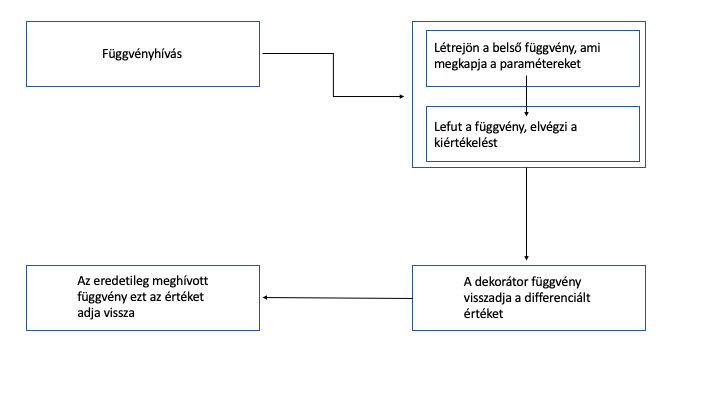
\includegraphics[width=\textwidth]{plots/numerical_derivation_decorator_explanation.png}
\subsection{Python csomagok}
Mint minden nyelvben, itt is tudunk importálni már készen levő csomagokat, amelyek tartalmaznak a célnak megfelelő osztályokat, azon belül metódusokat. Ha nincs feltelepítve a csomag, akkor a \textbf{pip install csomag-neve} paranccsal tehetjük meg azt.
Amint ezt megtettük, az \textit{import csomag-neve as alias-csomag-neve} módon importálhatjuk a kódunkba. A könnyebb olvashatóság érdekében szokás \textit{alias}-t használni, de nem szükséges.

\lstinputlisting[language=Python]{python-bevezetohoz-scriptek/import_template.py}
\section{Numerikus integrálás}
A numerikus integrálás nagyon fontos része a numerikus módszereknek. Egyrészről gyorsabban megkaphatjuk a határozott  integrál értékét, másrészről vannak olyan függvények, amelyeknek nem tudjuk kiszámolni papíron az integrál értéket, csak becsülni tudjuk alulról és/vagy felülről. A numerikus integrálás nagyban támaszkodik a kvadratúra képletekre.
\begin{definition}
Kvadratúra képletek általánosan

Az integrál értékét tudjuk közelíteni az ún. \textit{Kvadratúra képlettel}.\newline
\begin{equation*}
    \int_{a}^{b} f(x) dx \approx \sum_{k = 0}^{n} c_k f(x_k) = \sum_{k=0}^n \sigma_k \;\; , ahol\;\; x_i \in [a,b]
\end{equation*}

\end{definition}

Most nézzünk meg néhány kvadratúra képletet.
\subsection{Newton - Cotes formula}


Az integrálni való halmazt osszuk fel egyforma hosszúságúra, így vegyünk ekvidisztáns alappontokat.

\begin{equation*}
    x_k = a + hk \;\;, \;\;ahol \;\;k=0,1,...,n ,\;\; h = \frac{b-a}{n}
\end{equation*}
Írjuk fel az interpolációs kvadratúra képletet.
\newline
\begin{equation*}
    c_k = \int_a^{b} l_k(x) dx = h \int_0^{n} l_k (a+ht) dt = \frac{b-a}{n} \int_0 ^{n} \Pi_{j=0, j \neq k}^n \frac{t-j}{k-j} dt = \frac{b-a}{n} \frac{1}{k! (n-k)!} \int_0^n \Pi_{j=0}^{k-1} (t-j) \Pi_{j=k+1}^{n} (j-t) dt
\end{equation*}

\subsection{Összetett kvadratúra képlet}

\begin{equation*}
 \int_a^{b} f(x) dx = \sum_{j = 1} ^{m} \int_{a_{j-1}} ^{a_j} f(x) dx
\end{equation*}
 ahol $a_0 = a, a_m =b $

A baloldali részintegrált írjuk fel az interpolációs kvadratúra képlettel:
\begin{equation*}
\int_{a_{j-1}}^{a_j} f(x) dx \approx \sum_{k=0}^{r} c_{k,j}f(x_{k,j})
\end{equation*}

Innen helyettesítsünk vissza az eredeti képletbe
\begin{equation*}
\int_a^b f(x) dx \approx \sum_{j=1}^{m} \sum_{k=0}^{r} c_{k,j} f(x_{k,j})
\end{equation*}


\subsection{Érintő formula}

Az érintő formulához felfogjuk használni a függvények lineáris Taylor közelítését. Ezen felül vegyük az intervallum ekvidisztáns felosztását.
\begin{equation*}
   x_k = a + (k - \frac{1}{2})h ,\;\; ahol\;\; h = \frac{b-a}{n},\;\; k =1,...,n.
\end{equation*}



A Taylor közelítése a függvénynek a $[x_k-\frac{h}{2},x_k+\frac{h}{2}]$ intervallumon
\begin{equation*}
    f(x) \approx f(x_k)+f'(x_k)(x-x_k).
\end{equation*}

\begin{equation*}
\int_{x_k-\frac{h}{2}}^{x_k + \frac{h}{2}} \approx \int_{x_k - \frac{h}{2}}^{x_k + \frac{h}{2}} [f(x_k) + f'(x_k)(x-x_k)] dx = hf(x_k)
\end{equation*}
\newline
Innen pedig kapjuk, hogy
\begin{equation*}
\int_a^b = f(x) dx = \sum_{k=1}^n \int_{x_k - \frac{h}{2}}^{x_k + \frac{h}{2}} f(x)dx \approx h \sum_{k=1}^n f(x_k)
\end{equation*}



\subsection{A trapéz módszer és a Newton - Cortes módszer}
Írjuk fel a Newton - Cortes formulát n = 1 és k = 0 melett:
\begin{equation*}
c_0 = \frac{b-a}{1} \frac{1}{0!(1-0)!} \int_0^{1} \Pi_{j=0}^{0-j} \Pi_{j=0+1}^{1} (j-t) dt = (b-a) \int_0^1 (1-t) dt = \frac{b-a}{2}
\end{equation*}

\begin{equation*}
c_1 = \frac{b-a}{2}
\end{equation*}
Ekkor

\begin{equation*}
    \int_a^b f(x) dx \approx \frac{b-a}{2}[f(a) + f(b)] = \sum_{k=0}^{1} \frac{b-a}{2} f(x_k),\\
    \;\;ahol \;\;x_0 = a,\;\;x_1=b
    \;\;
\end{equation*}

Ez pedig pont a trapéz területe! Nézzünk erre egy példát :
\newline

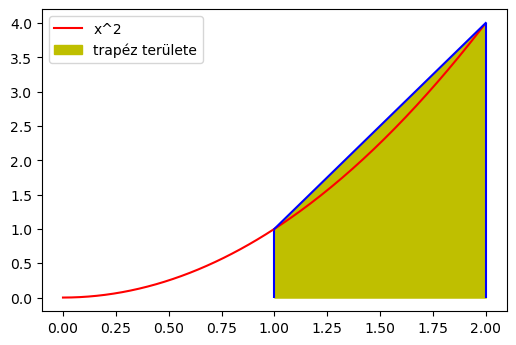
\includegraphics{plots/trapez_with_area.png}

Az integrál értéke ezen az intervallum 7/3.
\begin{center}
$\int_{1}^{2} x ^2 dx = \frac{7}{3}$
\end{center}
Azonban, ha ezen paraméterek között végezzük el a trapéz - területszámítást akkor 2.5 - t kapunk eredményként. Ezt onnan is láthatjuk, hogy a fenti ábrán a kék és piros vonal között még akad zöld terület. Azonban most számoljuk ki ezzel a módszerrel az integrál értékét az [1,1.5] és [1.5,2] intervallumokon. Ekkor eredményül 0.8125 és 1.5625, összesen 2.375 értéket kapunk, ami közelebb van a 7/3-hoz

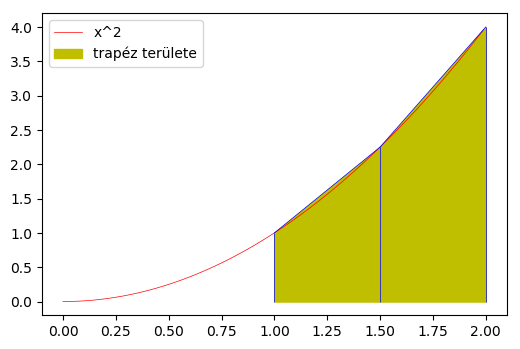
\includegraphics{plots/trapez_n=2.png}

\subsection{Python kódok a fejezethez}
A trapéz függvényben használjuk a globals() metódust. Ez a metódus visszaadja az összes olyan objektumot, amely az adott programunk futásakor belekerült a compilerbe(fordítoprogram). Ezek között lesznek azok a függvények, amiket megírtunk. A globals() egy dictionaryt ad vissza, amiben mi a függvény nevét fogjuk használni, mint kulcs.
\pagebreak
\lstinputlisting[language=Python]{functions.py}

\section{Szukcesszív approximációs módszer}

\begin{definition}{ODE}\\
Közönséges differenciálegyenletnek(Ordinary Differential Equation) nevezzük azokat az egyenleteket, amelyekben szerepel egy függvény egy változója szerinti deriváltja és célunk meghatározni a derivált függvényt.\\
Például
\begin{equation*}
    \frac{dx}{dt} (t) = cos(t)
\end{equation*}
\end{definition}

\begin{definition}Autonóm differenciálegyenlet\\
Írjuk fel a következő ODE-t:
\begin{equation*}
    f(x,y) = \frac{dy}{dt} = y'
\end{equation*}
Azokat a differenciálegyenleteket nevezzük autonómnak, amelyek nem függnek az x változótol a fent leírt egyenletben. Erre egy jó példa lehet a következő feladat.
\begin{equation*}
    \frac{dy}{dt} = f(y)
\end{equation*}
Ha t paramétert az időnek vesszük, akkor ebben az egyenletben azt láthatjuk, hogy nem függ az időtől az y megváltozása, mindig állandó a deriváltja, f(y) a változás időtől függetlenül.
\end{definition}

\begin{definition}Lineáris differenciálegyenlet\\
Lineáris differenciálegyenletnek nevezzük azokat a differenciálegyenleteket, ahol a jobb oldali f függvényt feltudjuk írni x deriváltjainak lineáris kombinációjaként.
Példa erre a következő:
\begin{equation*}
    a_1 x'(t) + a_2 x''(t) = f(t,x(t))
\end{equation*}
\end{definition}

\begin{definition}Nemlineáris differenciálegyenlet\\
Azokat a differenciálegyenleteket nevezzük \textit{nemlineáris differenciálegyenleteknek}, amelyben a deriváltak nem írhatóak fel egy lineáris kombinációban
\end{definition}

\begin{definition}Homogén differenciálegyenlet\\
Az olyan differenciálegyenlet, amely 0-val egyenlő, \textit{homogén differenciálegyenleteknek} nevezzük.
\end{definition}
\begin{definition}Nemhomogén differenciálegyenlet\\
Az olyan differenciálegyenleteket, amelyek nem 0-val egyenlőek \textit{nemhomogén differenciálegyenleteknek} nevezzük
\end{definition}
\begin{definition}{Kezdetiérték-feladat}\\
Vegyünk egy ODE problémát és adjunk meg hozzá egy (kezdeti) pont-függvény párost. Az ODE-t ezzel a tulajdonsággal ellátva kezdetiérték problémának  nevezzük
\begin{equation*}
    \begin{cases}
       x'(t) = f(t,x(t))\\
       x(t_0) = x_0 \\
    \end{cases}
\end{equation*}
\end{definition}
\begin{definition}{Lipschitz folytonosság}

\begin{equation*}
Legyen \;\;    f : \mathbb{R} \rightarrow \mathbb{R}, \; és \;\; L\; \;\in \mathbb{R}^+
\end{equation*}

Ha f minden x és y pontjára fennáll a következő
\begin{equation*}
    |f(x) - f(y)| \leq L |x-y|
\end{equation*}
egyenlőtlenség, akkor \textit{Lipschitz folytonosnak} nevezzük az f függvényt
\end{definition}
\begin{definition}{Kontrakció}\\
Legyen (X,$\textit{d}$) egy teljes metrikus tér. T leképezést $\textit{kontrakciónak}$ nevezzük X alaphalmazon, ha $\exists$ $q \in [0,1)$, hogy
\begin{equation*}
    d(T(x),T(y)) \leq q \textit{d}(x,y) \;\;,\forall x,y \in X
\end{equation*}
Pongyolán fogalmazva ezt jelenti, hogy azok a  Lipschitz folytonos függvények a kontrakciók, amelyekben az L Lipschitz konstans kisebb 1-nél
\end{definition}
\begin{theorem}[Banach-féle fixponttétel]
Legyen (X,$\textit{d}$) egy nemüres, teljes metrikus tér ellátva egy T kontrakcióval. Ekkor
\begin{equation*}
    \exists!\;\; x^* \in X : T(x^*) = x^*
\end{equation*}
\end{theorem}
\begin{proof}
Részletesen nem tisztázzuk a tétel bizonyítását, csak megemlítjük a főbb lépéseket.

\begin{equation*}
Legyen\;\;(X_n)_{n \in \mathbb{N}},\;\; x_n = T(x_{n-1}), \;\;x_0 \in X \;\;egy \;\; sorozat
\end{equation*}
Mivel T kontrakció, így igaz a következő egyenlőtlenség
\begin{equation*}
    d(x_{n+1},x_n) \leq q^n d(x_1,x_0)
\end{equation*}
Ha ezeket felhasználva elkezdünk \textit{n}-ben iterálni, könnyű belátni, hogy
\begin{equation*}
    \forall \;\; \epsilon >0 : \;\;d(x_j,x_k) j < \epsilon\;\;, \;\;j\neq k  \;\;
\end{equation*}
azaz  $(x_n)$ Cauchy  sorozat.
Mivel (X,d) metrikus tér teljesn ezért a sorozatunknak létezik határértéke, sőt ez a határéték pont T leképezés fix pontja lesz. A fix pont egyértelműségét igazolhatjuk, ha indirekt feltesszük, hogy van másik fix pont.
\end{proof}
%https://en.wikibooks.org/wiki/Ordinary_Differential_Equations/The_Picard–Lindelöf_theorem
\begin{theorem} [Picard - Lindenlöf] \\
Legyen I =[a,b] egy intervallum , és egy f függvény,

\begin{equation*}
f :  I \times \mathbb{R}^n \rightarrow \mathbb{R}^n
\end{equation*}
Legyen x' pedig egy ODE
\[
x'(t) = f(t,x(t))
\]
Ha f Lipschitz folytonos x(t)-ben, akkor az ODE-nek létezik egyértelmű megoldása [a,a + $\epsilon$]
intervallumon minden
\[
x(0) = x_0 \in \mathbb{R}^n, \epsilon < \frac{1}{L}
\] halmazra és L pedig x(t) Lipschitz konstansa
\end{theorem}
\begin{proof}
Írjuk fel ezt egy kezdeti-érték feladatra
\begin{equation*}
    \begin{cases}
       f :  I \times \mathbb{R}^n \rightarrow \mathbb{R}^n , t \in [a,a + \epsilon]\\
       x'(t) = f(t,x(t))\\
    \end{cases}
\end{equation*}

Ez a Newton - Leibniz tétel miatt pedig erre az alakra hozható:
\begin{equation*}
    \forall t \in [a, a +\epsilon] : x(t) = x_0 + \int_{a}^{t} f(s,x(s)) ds
\end{equation*}
 ahol pedig $\epsilon < \frac{1}{L}$. Eszerint x(t) fixpontja a következő függvénynek :

 \begin{equation*}
     T : \mathcal{C}([a, a +\epsilon]) \rightarrow \mathcal{C}([a, a +\epsilon]), T(x,t) := x_0 + \int_a^t f(s,x(s)) ds
 \end{equation*}
 T kielégíti a Lipschitz folytonosságot, mivel
 \begin{equation*}
    \begin{split}
     \lVert T(x,t) - T(y,t) \rVert =\lVert \int_a^t f(s,x(s)) ds - \int_a^t f(s,x(s)) ds \rVert &
     \leq \int_a^t \lVert f(s,x(s)) - f(s,y(s)) \rVert ds \leq \int_a^t L \lVert x(s) - y(s) \rVert &
     \leq (t-a) L \lVert x-y\rVert_{\infty} \leq \epsilon L \lVert x - y \rVert_{\infty}
     \end{split}
 \end{equation*}

 Mivel T pedig kontrakció, így a Banach-féle fixpont tétel alkalmazható,amivel igazoltuk a létezését a megoldásnak. Továbbá felhasználva a Peano-egyenlőtlenséget megkapjuk az egyértelműséget is.
\end{proof}
\begin{definition}[Szukcesszív approximációs módszer]
Vegyük a következő kezdetiérték problémát
\begin{equation*}
    \begin{cases}
       x'(t) = f(t,x(t))\\
       x(a) = b
    \end{cases}
\end{equation*}
Fentebb tárgyaltuk a Picard-Lindelöf tételnél, hogy a Newton - Leibniz tétel miatt fennáll a következő
egyenlőség: \newline
\begin{equation*}
    x(t) = x(0) + \int_a^t f(s,x(s)) ds
\end{equation*}
Ekkor vegyük az \[x_0(t) = b\] állandót, majd kezdjünk el előre iterálni a következő képlet alapján:
\begin{equation*}
    x_{n + 1}(t) = b + \int_a^t f(s,x_n(s)) ds
\end{equation*}
\end{definition}

\begin{example}[Exponenciális függvény]
\begin{equation*}
    \begin{cases}
       y'(t) = y\\
       y(0) = 1
    \end{cases}
\end{equation*}
Kezdjünk el lépkedni.
\begin{equation*}
    y_1(t) = 1 + \int_0^x 1 dt = 1 + x
\end{equation*}
\begin{equation*}
    y_2(t) = 1 + \int_0^x 1+t dt = 1 + x + \frac{x^2}{2}
\end{equation*}
\begin{equation*}
    y_3(t) =  1 + x + \frac{x^2}{2} + \frac{x^3}{6}
\end{equation*}
\begin{equation*}
    y_4(t) = 1 + x + \frac{x^2}{2} + \frac{x^3}{6} + \frac{x^4}{24}
\end{equation*}
\begin{equation*}
    y_{\infty}(t) = exp(x)
\end{equation*}
\end{example}
\subsection{Python kódok a fejezethez}
\lstinputlisting[language=Python]{fokozatos_kozelitesek/successive.py}
\section{Runge-Kutta módszer}
A Runge-Kutta algoritmusok az egyik legelterjedtebb megoldó módszerek a numerikus analízis eszköztárában, mivel 'olcsó' a használatuk, nem igényelik a függvények deriváltjainak az ismeretét és mégis elfogadható pontossággal műküdnek (ez például nem mondható el feltétlen az Euler módszerről). A módszer a nevét két német matematikusról kapta, nevesen Carl Runge és Wilhelm Kuttáról.

\subsection{Euler módszer}
Alapvetően nem fogjuk használni az Euler módszert, azonban mindképp említést kell tennünk róla, mivel a Runge - Kutta módszer erre épít. Ez nagyon szemléletes megoldási metódus, azonban nem praktikus ha általánosan akarunk felírni egy kódot hozzá, mert épít a deriváltakra.\\

Vegyünk egy kezdetiérték problémát és hozzá egy lépésközt.
\begin{equation*}
    \begin{cases}
       x'(t) = f(t,x(t))\\
       x(a) = b \\
       t_i = a + ih , i \in \{0,1,...,N\}
    \end{cases}
\end{equation*}

Itt pedig a lépésköz pedig legyen \[h = \frac{b-a}{N} = t_i - t_{i-1} \]

Használjuk fel a Taylor sorbafejtést másodrendben x-re.
\begin{equation*}
    x(t_{i+1}) = x(t_i) + h x'(t_i) + \frac{h^2}{2} x''(\xi_i) \;\;,\;ahol \;\;\xi _i \in (t_i, t_{i+1})
\end{equation*}

Ezek alapján pedig láthatjuk, hogy az algoritmust a következőképpen írhatjuk fel:
\begin{equation*}
    \begin{cases}
        x_0 = \alpha \\
        x_{i+1} = x_i + h f(t_i,x_i) \;\;\forall i \in{0,1,...,N-1}
    \end{cases}
\end{equation*}
\subsection{RK4}
Runge - Kutta módszerekből sokat alkottak az utóbbi időkben. Ha egyszerűen próbáljuk meg megközelíteni ezeknek a megoldó algoritmusoknak a felépítését, akkor észrevehetjük, hogy ahányad rendű Runge - Kutta módszert használunk, annyiad rendű Taylor sor közelítést használunk.Mi most a Runge-Kutta negyedfokó közelítését használjuk, amire a szakirodalomban sokszor csak 'RK4' módon hivatkoznak. A 4-ed rendű közelítés a következő formulából vezethető le:
\begin{equation*}
\begin{split}
      y_{t+h} = y_t + h \sum_{i=1}^{s} a_i k_i + \mathcal{O}(h^{s+1}),\\
      ahol\;\;k_i = y_t + h \sum_{j=1}^{s} \beta_{i,j} f(k_j,t_n + \alpha_ih)
\end{split}
\end{equation*}

A képlete pedig s=4 mellett:
\begin{equation*}
\begin{cases}
        x_0 = \alpha \\
        k_1 = h f(t_i,w_i) \\
        k_2 = h f(t_i + \frac{h}{2}, w_i + \frac{1}{2} k_1) \\
        k_3 = h f(t_{i + 1} + \frac{h}{2}, w_i + \frac{1}{2} k_2) \\
        k_4 = h f(t_{i + 1}, w_i + k_3)\\
        w_{i+1} = w_i + \frac{1}{6}(k_1 + 2k_2 + 2k_3 + k_4)\\
        t_{i+1} = \alpha + ih
\end{cases}
\end{equation*}
Ezt pedig már tudjuk iterálni i-ben egy rögzített h mellett. Ennek a közelítésnek előnye, hogy a hibahatára már elfogadható és nem igényel annyira sok számítást, mint egy magasabb rendű közelítés
\subsection{Példa feladatok}
\begin{example} [Konstans együtthatós lineáris ODE]
Legyen \\
\begin{center}
   \begin{cases}
    x' = 5x - 3 \\
    x(0) = 1
   \end{cases}
\end{center}
Ennek a kezdetiérték feladatnak az analitikus megoldása a következő:
\begin{equation*}
\begin{split}
        \frac{dx}{dt} &= 5x - 3 \\
        \frac{1}{5x-3} dx &= 1\; dt \\
        \int \frac{1}{5x-3} dx &= \int 1\; dt \\
        \frac{1}{5} ln|5x-3| &=t + C \\
        5x -3 &=e^{5(t + C)} \\
        x &= \frac{e^{5(t+C)} + 3}{5}
\end{split}
\end{equation*}
Mivel x(0) = 1, így
\begin{equation*}
    x(0) = \frac{e^{0+C} + 3}{5} = \frac{e^{5C}+3}{5} = 1
\end{equation*}
\begin{equation*}
    e^{5C} + 3 = 5
\end{equation*}
\begin{equation*}
    5C = ln2
\end{equation*}
\begin{equation*}
    C = \frac{ln2}{5}
\end{equation*}
Tehát a keresett függvény :
\begin{equation*}
    x(t) = \frac{e^{5(t + \frac{ln2}{5})} + 3}{5}
\end{equation*}
Nézzük meg mennyit ad a függvény a t=1 pontban:
\begin{equation*}
    x(1) = \frac{e^{5(1 + \frac{ln2}{5})} + 3}{5} \approx 59.9653
\end{equation*}
A függvényünk h = 0.1-es lépésköz mellett 59.8632 -es értéket adott. Ha h = 0.01, akkor sok tizedesjegyig megegyezik az eredmény. Azonban nem feltétlen szabad a megoldó algoritmusban h - t igazán kicsinek venni, mert könnyen a visszajára fordulhat. (Ez például függ attól, hogy hány bites a processzor. Nagyon nagy irodalma van az optimális értékek beállítására, azonban most ez a szakdolgozat ezzel nem foglalkozik)
\end{example}

\begin{example}[Folytonos kamatozás]
Tegyük fel, hogy elhelyezünk egy bankban konstans kamatláb mellett egy betétet folytonos kamatozás mellett. Tudjuk, hogy a folytonos kamatozás képlete
\begin{equation*}
    e^{rt},\;\; ahol \; r\; a\; kamatláb \;és\;t\; az \;idő
\end{equation*}
Ezt kifejezhetjük egy kezdetiérték probléma alakban is a következő módon : \\
\begin{center}
  \begin{cases}
        x' = rx \\
        x(0) = 1
  \end{cases}
\end{center}
Ennek a megoldása pedig pont visszaadja a fentebb írt képletet: \\
\begin{equation*}
    \frac{dx}{dt} = r x
\end{equation*}
\begin{equation*}
    \frac{1}{x} dx = r dt
\end{equation*}
\begin{equation*}
    \int \frac{1}{x} dx = \int r dt
\end{equation*}
\begin{equation*}
    ln|x| = rt + c
\end{equation*}
\begin{equation*}
    x = e^{rt + c}
\end{equation*}
Mivel a kezdetifeltétel x(0) = 1, így c = 0 és visszakapjuk az eredeti képletet\\

Nézzük meg mennyi lehet x(1), úgy hogy r = 0.1 a kamatláb. A képlet szerint tudjuk, hogy
\begin{equation*}
    e^0.1 = x(1) = 1.105170918...
\end{equation*}
Ha ezt az értéket beheleyttesítjük a numerikus RK4-es függvényünkbe, akkor az x(1) = 1.1051709180665144 eredményt kapjuk 0.1-es lépésköz mellett. Ennél példánál a negyedrendű Runge-Kutta módszer elég pontos eredményt adott
\end{example}


\begin{example}[Másik példa]\\
Legyen \\
\begin{center}
   \begin{cases}
    x' = \frac{x^3}{3} \\
    x(0) = 3
   \end{cases}
\end{center}
egy kezdeti érték feladat. Ennek a megoldása pedig
\begin{equation*}
    x(t) = \frac{3}{\sqrt{1-6t}}
\end{equation*}

Az analitikus eredmény t = 0.1 pontban :
\begin{equation*}
    x(0.1) \approx 4.7434
\end{equation*}
A Runge-Kutta módszer eredménye úgyszintén 4.7434.
\end{example}

\begin{example} [Egy nehezebb elsőrendű feladat]
Nézzük a következő feladatot: \\
\begin{center}
    \begin{cases}
     x' = \frac{1}{x(9 + 4 t^2)} \\
     x(0) = 1
    \end{cases}
\end{center}
Ennek a feladatnak az analitikus megoldása :
\begin{equation*}
    x(t) = \sqrt{\frac{1}{3} arctg(\frac{2t}{3}) + 1}
\end{equation*}
\begin{equation*}
   x(0) = \sqrt{\frac{1}{3} arctg(\frac{0}{3}) + 1} = 1
\end{equation*}
A numerikus eredmény pedig: 1.0110.
Ez az első feladat, ahol jelentős az eltérés, nevesen kb. 0.01
\end{example}
A Runge-Kutta és minden egyéb numerikus módszer tehát nem arra jó, hogy meghatározzuk analitikusan , képlettel a függvény formáját, hanem egy közelítést ad arra, hogy mi lehet a keresett függvény \textbf{értéke az adott pontban.}
\subsection{Eredmények összevetése}
A Runge Kutta módszert kevesebb lépésből mindig pontosabb eredményt adott, ez is egy oka , amiért ez terjedt el inkább az iparban. Azonban most az egyszerűség kedvéért az Euler módszer eredményeit úgy közlöm ebben a táblázatban, hogy nem ugyanakkora energiabefektetéssel készültek, mint az RK4-es párjai. Ez a gyakorlatban azt jelenti, hogy minden esetben addig emelgettem az iterációs számokat, ameddig be nem állt az adott értékre, amitől már számottevően nem tért el a továbbiakban. Ezek után a legjobb Euler módszer eredményeket tettem bele a táblázatba, míg az RK4-es eredmények konzistensen nem változtak felépítésüket tekintve, nem nyúltam bele sehogy sem a megoldó algoritmus paramétereibe.
\begin{table}[H]
\begin{tabular}{|l|l|l|l|}
\hline
                           & Analitikus megoldás & Runge Kutta & Euler módszer \\ \hline
Konstans együtthatós példa & 59.9653             & 59.9652     & 59.2302       \\ \hline
Kamatláb példa             & 1.1051              & 1.1051      & 1.1051        \\ \hline
Harmadfokú példa           & 4.7434              & 4.7434      & 4.7409        \\ \hline
Bonyolultabb példa          & 1.0000              & 1.0110      & 1.0936        \\ \hline
\end{tabular}
\end{table}
Látni az eredményeken, hogy az RK4 jobb eredményekre vezetett az Euler módszernél. A következő néhány képen pedig bemutatjuk a két módszer pontosságát. Az első képen a konstans együtthatós példa szerepel 100-as és 200-as lépésszámok mellett. Látni, hogy az RK4 kevesebb lépésből közelebb került a megoldáshoz.

\includegraphics[width=\textwidth, height=290pt]{RK4/plotok/konstans_rk4=100_euler=200.png}
A második képen pedig látni, hogy ugyanakkora lépésszám mellett ebben az esetben pedig pontosabb eredményt adott az RK4.

\includegraphics[width=\textwidth]{RK4/plotok/konstans_mindketto_200.png}

Természetesen úgy kerek, ha megmutatjuk, hogy más esetekben ezektől függetlenül nehéz leolvasni az ábráról, hogy van eltérés az eredmények között. Ilyen volt az a példa, ahol a kamatláb esetet vizsgáltuk. Itt a piros vonalat meg kellett vastag0tani, mert végig fej fej mellett haladt a két vonal

\includegraphics[width=\textwidth, height=290pt]{RK4/plotok/kamatlab_step=100.png}
\subsection{Magasabb rendű egyenletek megoldása}
A Runge Kutta módszerek működnek magasabb rendű differenciál egyenletek megoldására is. Alapvetően nagyon hasonlít az elsőrendű megoldó képlethez. Amikor analitikusan szeretnénk megoldani egy magasabb rendű egyenletet, akkor általában úgy szoktuk megoldani, hogy bevezetünk új változókat az egyes deriváltakra és ezt folytatva redukáljuk a problémát egy olyan feladatra, aminek már ismerjük a megoldási lehetőségét, lehetőségeit. Ha letudtuk redukálni a problémát elsőrendű alfeladatokra, akkor azok össze lesznek kapcsolódva a bizonyos változókban és erre tudjuk alkalmazni, például a Runge Kutta módszert (nem feltétlen csak a negyed rendű közelítést).\newline
Nézzük meg példának egy (általánosan felírt) másodrendű differenciál egyenlet megoldását az RK4 módszerrel.
\begin{center}
    \begin{cases}
    x'' = f(t,x,x') \\
    x(t_0) = x_0 \\
    x'(t_0) = z_0
   \end{cases}
\end{center}
Vezessük be a következő változókat:
\begin{equation*}
    z = x'
\end{equation*}
\begin{equation*}
    z' = x'' = f(t,x,x') = f(t,x,z)
\end{equation*}

\begin{center}
    \begin{equation*}
        x = &
        \begin{bmatrix}
            x_n \\
            z_n
        \end{bmatrix}
    \end{equation*}
\end{center}
\begin{center}
    \begin{equation*}
        K_i = &
        \begin{bmatrix}
            K_i \\
            L_i
        \end{bmatrix}
    \end{equation*}
\end{center}
\begin{equation*}
    K_1 = h Z_n , \;\;L_1 = h f(t_n, x_n, Z_n)
\end{equation*}

\begin{equation*}
    K_2 = h (Z_n + \frac{L_{1}}{2}) , \;\;L_2 = h f(t_n + \frac{h}{2}, x_n+ \frac{K_{1}}{2}, Z_n + \frac{L_{1}}{2})
\end{equation*}

\begin{equation*}
    K_3 = h (Z_n + \frac{L_{2}}{2}) , \;\;L_3 = h f(t_n + \frac{h}{2}, x_n+ \frac{K_{2}}{2}, Z_n + \frac{L_{2}}{2})
\end{equation*}

\begin{equation*}
    K_4 = h (Z_n + L_{1}) , \;\;L_4 = h f(t_n + h, x_n+ K_{3}, Z_n + L_{1})
\end{equation*}

Ezután pedig a kettő megoldandó egyenletet az előbbiekhez nagyon hasonlóan elkezdjük iterálni a következő képletek alapján:

\begin{equation*}
    x_{n+1} = x_n + \frac{1}{6}(K_1 + 2K_2 + 2K_3 + K_4)
\end{equation*}

\begin{equation*}
    Z_{n+1} = Z_n + \frac{1}{6}(K_1 + 2K_2 + 2K_3 + K_4)
\end{equation*}
\subsection{Python kódok a fejezethez}
Elsőre itt találhatjuk meg a Runge Kutta numerikus módszer implementációját néhány példával, hogy követhető legyen a használata.
\lstinputlisting[language=Python]{RK4/rk4.py}

Itt pedig az Euler módszer általam megírt változatát találhatjuk.
\lstinputlisting[language=Python]{RK4/euler_method_template.py}
\section{Stabilitás elméleti kitekintés}
A stabilitás elmélet egy nagy része a differenciálegyenletek témakörének. Ebben a dolgozatban szeretnénk egy kicsi betekintést nyerni ebbe a világba. Első körben tisztázzunk néhány definíciót
\subsection{Alapfogalmak}
A fejezetben végig vegyük adottnak a
\begin{equation*}
    x' = f(t,x)
\end{equation*}
függvényt, ahol
\begin{equation*}
    f: I \times \Omega \rightarrow \mathbb{R}^n \\
\end{equation*}
\begin{equation*}
    (t,x) \rightarrow f(t,x)
\end{equation*}
\begin{equation*}
    I=(t,\infty)
\end{equation*}
\begin{equation*}
    0 \in I
\end{equation*}
\begin{definition}[Egyensúlyi pont]
A fent bevezetett függvény mellett az
\begin{equation*}
    x' = 0 = f(t,x)
\end{equation*}
pontot egyensúlyi pontnak nevezzük
\end{definition}
A továbbiakban az
\begin{equation*}
    (x_0,t_o) \in I \times \Omega
\end{equation*}
legyen olyan intervallum, hogy f-nek egy megoldása legyen csak

\begin{definition}
Jelöljük a következő módon a vektorok felsőbecslésének halmazát :
\begin{equation*}
    B_{\rho} : = \{ x \in \mathbb{R}^n: \lVert x \rVert < \rho \}
\end{equation*}
\end{definition}
A következő néhány definíció fontos alapfogalmai a stabilitáselméletnek, így minnél pontosabb megfogalmazásra törekedünk, a [Sárga könyv] alapján. Amikor egy stabilitás fajtát tárgyalunk, azt a megoldásra kell értelmezni. Tehát ha megállapítjuk, hogy valami stabil, akkor azt arra fogjuk érteni, hogy a megoldás stabil.
\begin{definition}[Megoldás legbővebb halmaza]
Jelölje $J^+$ az x legbővebb lehetséges megoldás halmazát. Természetesen
\begin{equation*}
    J^+ \subseteq [t_0, \infty]
\end{equation*}
\end{definition}
\begin{definition} [Stabilitás]
\begin{equation*}
    \forall \epsilon > 0 \;-hoz\;\;és\;\;t_0 \in I \;-re\; \exists\;
    \delta >0\;,\;hogy\;\; \forall x_0 \in B_{\delta} \;és\; t \in J^+ \;esetén
\end{equation*}
\begin{equation*}
    \lVert x(t,(t_0,x_0)) \rVert < \epsilon
\end{equation*}
\end{definition}

\begin{definition}[Instabilitás]
Az instabil, ami nem stabil.
\end{definition}

\begin{definition}[Vonzás (attraktivitás)]
Az x' = f(t,x) x=0 megoldását vonzónak nevezzük, ha
\begin{equation*}
    \forall t_0 \in I \; esetén\; \exists\; \eta = \eta(t_0)
\end{equation*}
\begin{center}
    és
\end{center}
\begin{equation*}
    \forall \epsilon > 0\; esetén \;és\; \forall \; \lVert x_0 \rVert < \eta \;-ra \; \exists \; \sigma = \sigma(t_0,\epsilon,x_0) > 0
\end{equation*}
\begin{center}
    olyan módon, hogy
\end{center}
\begin{equation*}
    \forall \; t_0 + \sigma \leq t \;és\; t \in J^+ \;esetén \; \lVert x(t,t_o,x_0) \rVert < \epsilon
\end{equation*}
\end{definition}
\begin{definition}[Egyenletes stabilitás]
\begin{equation*}
    \forall \; \epsilon > 0 \; mellett \; \exists \; \delta  = \delta(\epsilon) \;olyan \;módon,\;hogy
\end{equation*}
\begin{equation*}
    \lVert x(t,(t_0,x_0)) \rVert < \epsilon
\end{equation*}
\begin{equation*}
    \forall t_0 \in I, \forall \; \lVert x_0 \rVert < \delta,
    \forall \; t_0 \leq t-ra \;teljesül
\end{equation*}
\end{definition}

\begin{definition}[Egyenlően vonzó]
\begin{equation*}
    \forall \; t_0 \in I \; esetén \; \exists \eta = \eta(t_0).
\end{equation*}
\begin{center}
    és
\end{center}
\begin{equation*}
    \forall \epsilon > 0 \; mellett \; \exists \; \sigma = \sigma(t_0,\epsilon) > 0
\end{equation*}
\begin{center}
    olyan módon, hogy
\end{center}
\begin{equation*}
    t_0 + \sigma \in J^+ : \lVert x(t,(t_0,x_0)) \rVert < \epsilon
    \;
\end{equation*}
\begin{equation*}
     \forall \; \lVert x_0 \rVert < \eta
\end{equation*}
\begin{equation*}
     \forall t_0 + \sigma \leq ; \; t \in J^+
\end{equation*}
\end{definition}

\begin{definition}[Egyenletesen vonzó]
\begin{equation*}
  \exists \eta > 0 \;és \; \forall \; \epsilon > 0 \;mellett \; \exists \sigma = \sigma(\epsilon)
\end{equation*}
\begin{center}
olyan módon, hogy $t_0 + \sigma \in J^+,$ és
\end{center}
\begin{equation*}
    \lVert x(t,(t_0,x_0)) \rVert < \epsilon
\end{equation*}
\begin{equation*}
    \forall \lVert x_0 \rVert < \eta, \;és
\end{equation*}
\begin{equation*}
    t_0 + \sigma \leq t, t \in J^+
\end{equation*}
\end{definition}

\begin{definition}[Globálisan vonzó]
\begin{equation*}
    \forall \eta > 0 \;és\; \forall t_0 \in I\;esetén
\end{equation*}
\begin{equation*}
     \lim_{t\to 0} x(t,(t_0,x_0))  \rightarrow 0
\end{equation*}
és emellé mind $t_0$-ban ,mind $x_0$-ban egyenletes a konvergencia
\end{definition}

A globálisan vonzó megoldás definíciója után ésszerű lehet kimondani ,hogy milyen lehet egy pont vonzási körzete, jelesül az origóé.

\begin{definition}[Origó vonzási körzete vagy attraktivitási tartománya]
Jelölje A() a következő halmazt :
\begin{equation*}
    A(t_0) := \{ x_0 \in \Omega : \lim_{t\to 0} x(t,(t_0,x_0))  \rightarrow 0 \}
\end{equation*}
Ha ez $t_0$-tól független, akkor egyenletesnek mondjuk a vonzási körzetet.
\end{definition}

Az alapvető definíciók mellé még mondjunk ki 4 megoldási jellemzhetőséget, amelyek egymásnak finomításai.

\begin{definition}[Aszimptotikus stabilitás]
Az x' = f(t,x) függvénynek az x = 0 megoldási aszimptotikusan stabil, ha stabil és vonzó
\end{definition}

\begin{definition}[Egyenlően aszimptotikusan stabil]
Minden megoldás egyenlően aszimptotikusan stabil, ha stabil és egyenlően vonzó
\end{definition}

\begin{definition}[Egyenletesen aszimptotikusan stabil]
Egyenletesen aszimptotikusan stabilnak nevezzük azokat a megoldásokat, amelyek egyenletesen stabilok és egyenletesen vonzóak
\end{definition}

\begin{definition}[Globálisan egyenletesen aszimptotikusan stabil]
Globálisan egyenletesen aszimptotikusan stabil hívjuk azokat a megoldásokat, amelyek egyenletesen stabil és egyenletesen globálisan vonzó
\end{definition}
\subsection{Lineáris algebrai kitekintő}
Amikor egy rendszer stabilitását vizsgáljuk, akkor nagyban kell támaszkodnunk a különböző lineáris algebrai ismereteinkre.Ezért a következőkben kimondunk néhány tételt és definíciót, amelyek segítenek megérteni a különböző tételeket amelyek a stabilitásvizsgálathoz kapcsolódnak.

\subsubsection{Mátrix az exponenciális függvényben}
Az egydimenziós exponenciális függvény és a mátrixokra kiterjesztett változata képletben nem mutat eltérést, sőt a különböző konvergencia megállapítások is hasonlítanak egymásra.
\begin{definition}[Mátrixokra kiterjesztett exponenciális függvény]
Legyen X egy négyzetes mátrix. Ekkor a következő módon értelmezzük a mátrix kitevőt az exponenciális függvényben.
\begin{equation*}
    exp(X) := \sum_{k=0}^{\infty} \frac{X^k}{k!}
\end{equation*}
\end{definition}
\begin{theorem}
A mátrixokra kiterjesztett exponenciáliss függvény tartja a következő tulajdonságokat:
        \begin{equation*}
            e^{A+B} = e^A + e^B
        \end{equation*}

        \begin{equation*}
            e^{-A} e^{A} = I
        \end{equation*}

        \begin{equation*}
            \frac{d}{dt} e^{tA} = A e^{tA}
        \end{equation*}
\end{theorem}
\subsubsection{Sajátértékek és sajátvektorok}
\begin{definition}[Sajátérték]
Legyen A egy lineáris operátor (mátrix). Vegyünk emellé egy nem nem nulla vektort. Ekkor a $ \lambda \in \mathbb{C}$ az A mátrix sajátértéke, ha kielégíti a következő egyenletet
\begin{equation*}
    Ax = \lambda x
\end{equation*}
Szokás átrendezni ezt az egyenletet és a következő formában megadni:

\begin{equation*}
    (A-\lambda I)x= \textbf{0},
\end{equation*}
ahol I természetesen az egységoperátor (mátrix)
\end{definition}
A lambda skalárt a komplex számok felett definiáltuk, hogy ne sértsük meg az általánosságot, de ez működik a valós számtest felett is (ami a komplex számtest részhalmaza).
\begin{definition}[Sajátvektor]
Legyen A egy lineáris operátor , jelesül egy mátrix .Az A mátrix minden olyan nem zérus \mathbb{x} vektorát sajátvektorának nevezzük, amelyre fenáll a következő egyenlőség
\begin{equation*}
    Ax = \lambda x
\end{equation*}
\end{definition}
A sajátvektor skalárszorosa is sajátvektor marad ugyanazzal a sajátértékkel.

Tehát a sajátérték és a sajátvektor fogalmak nagyon szoros kapcsolatban állnak egymással.

\subsubsection{Sajátértékek meghatározása}
Amikor meg kell határoznunk egy mátrix sajátértékeit, akkor azt alapvetően több féle képpen tudjuk megtenni. Azonban amikor ezeket papíron végezzük el, az a mátrix dimenziójának növekedésével nem lineárisan megnöveli a számítási igényt, ezzel pedig méginkább nagyobb lesz az esély, hogy valahol elrontjuk a számolást és ezzel a végeredményt. A lineáris rendszerek stabilitásvizsgálatában központi szerepet játszanak a sajátértékek, így ebben az alfejeztben körbejárunk ezt numerikus megközelítésből.

Amikor felakarjuk írni egy mátrix sajátértékeit, akkor azt általában a karakterisztikus polinom gyökeinek megoldásaiként szoktuk megkapni.

\begin{equation*}
    det(A-\lambda I) = 0
\end{equation*}

Ez egy nxn-es mátrix esetén egy legfeljebb n-edfokú polinomot eredményet.
\begin{equation*}
    p(\lambda) = \sum_{i=0}^{n} c_i \lambda^i
\end{equation*}
Polinomokra mindig fogunk megoldást találni, így a sajátértékek is megfogjuk találni.

Elsőre  érdekességképp bemutatjuk a hatványmódszert (power method). Ez a módszer azért érdekes, mert csak a domináns sajátértékét számolja ki egy mátrixnak. Az alapgondolatát Richard von Mises és H. Pollaczek-Geiringer mutatták be még az 1920-as években. Ez egy iteratív eljárás, ami lépésről lépésre konvergál a domináns sajátérték felé. Gyakorlati haszna olyan mátrixok esetében van, amiben rengeteg a 0. Ez leginkább csak a számítógépes problémák esetében kerül elő. Talán a leghíresebb algoritmus, ami épít erre az a Google PageRank algoritmusa. Ez pont ideális, mert ha a honlapok kapcsolati gráfját mátrix formában írjuk fel, akkor meglehetősen sok 0 elemet fog tartalmazni (sparse matrix) és ekkor már ideális megközelítés lehet a hatványmódszer.

Az algoritmus maga úgy működik, hogy veszünk egy diagonalizálható mátrixot (A) és mellé egy \textbf{b} vektort. Ez a vektor legyen véletlen vagy ha tudunk valamit a problémáról, akkor közelítése a domináns sajátvektort.

Ezután a következő lépéssorozatot iteráljuk, addig ameddig beállítjuk, hogy k milyen indexhalmazon megy végig:
\begin{equation*}
    b_{k+1} =\frac{A b_{k}}{\lVert A b_{k} \rVert}
\end{equation*}
A norma alatt a szokásos euklideszi normát értjük. A módszer azonban nem feltétlen lesz konvergens, különböző feltételeknek kell teljesülnie ahhoz, hogy azzá váljon adott mátrixra.

Erre nézzünk egy rövid Python kódot, ami elvégzni ezt a lépéssorozatot.:

\lstinputlisting[language=Python]{linalg/eigenvals.py}

Ha azonban minden sajátértékre szükségünk van, akkor megprobálhatunk a QR algoritmussal haladni, aminek az alapjait az 1950-es években John G. F. Francis és Vera N. Kublanovskaya dolgozták ki egymástól függetlenül.

Végezetül nézzük meg a \textit{numpy} csomag sajátérték és sajátvektor kiszámító függvényt.

A függvény bemenete egy mátrix (numpy arrayt adunk meg most), a kimenete pedig a sajátértékek listája és a sajátvektorok listája.

Példaként nézzük meg a
\begin{bmatrix}
10 & 20\\
30 & 40
\end{bmatrix}
mátrix sajátértékeit és sajátvektorait.
\begin{equation*}
    \lambda_1 = -5 \sqrt{33}+25 \approx -3.7228
\end{equation*}
\begin{equation*}
    \lambda_2 = 5 \sqrt{33} + 25 \approx 53.7227
\end{equation*}

\begin{equation*}
    v_1 = [-1.4574 , 1]
\end{equation*}
\begin{equation*}
    v_2 = [0.4574 , 1]
\end{equation*}
és ezek a sajátvektorok konstanszorosai a numpy.linalg.ein() által megadott eredményeknek
\lstinputlisting[language=Python]{linalg/numpy_linalg_eigenvals.py}
Szerencsére ez a függvény a numpy.linalg csomagból azt is meghatározza, ha egy mátrix sajátértéke komplex szám, amire nagy szükségünk lesz a lineáris rendszerek stabilitásának vizsgálatakor.


A következő alfejezetben nézzünk meg néhány tételt, amelyek a stabilitás meghatározására vonatkoznak a lineáris esetekben
\subsection{Rendszerek stabilitása linearizálással}

\begin{theorem}
Legyen A négyzetes mátrix diagonalizálható, és

\begin{equation*}
    \lambda_{1}, \lambda_{2}, \lambda_{3}, ... ,\lambda_{r}
\end{equation*}
a különböző sajátértékei. Ha P jelöli a következő halmazt,
\begin{equation*}
    P_k := \prod_{j \neq k, 1 \leq j \leq r} \frac{A - \lambda_{j} I} {\lambda_{k} - \lambda_{j}}
\end{equation*}
akkor
\begin{equation*}
    P_k^2 = P_k
\end{equation*}
és
\begin{equation*}
    \sum_{k=1}^r P_k = I
\end{equation*}
\end{theorem}

Ez a tétel azért volt fontos, mert ennek a segítségével könnyen fogjuk tudni kezelni egy mátrix exponenciális eredményét.

\begin{theorem}
Legyen A egy négyzetes és diagonalizálható mátrix, $\lambda_1,...,\lambda_r$ pedig az összes különböző sajátértéke. Ekkor, az elöző tétel jelölését követve fenáll a következő egyenlőség
\begin{equation*}
    e^{tA} = \sum_{k=1}^r e^{\lambda_k t} P_k
\end{equation*}
\end{theorem}
A következő néhány tétel erejéig a vizsgálandó mátrix alatt az \textbf{x'} = f(\textbf{x}) -et értjük
\begin{theorem}
Ha az f'(a) \in \mathbb{R} ^ {n x n} \;\;mátrixra \;\;
\begin{equation*}
    \forall \lambda_i : Re(\lambda_i) < 0
\end{equation*}

akkor a pont aszimptotikusan stabil megoldása a feladatnak
\end{theorem}

\begin{theorem}
Ha az f'(a) mátrixnak

\begin{equation*}
    \exists \lambda_i : Re(\lambda_i) > 0,
\end{equation*}
 akkor a pont instabil egyensúlya a feladatnak
\end{theorem}
\section{Perturbáció elméleti megközelítés}
...Ezzel a résszel a stabilitás után fogok foglalkozni...
\section{Numba}
Mikroökonómia órán, majd részletesebben egyensúlyelméleten elhangzott, hogy egy vállalat a profitmaximumát többek között akkor tudja elérni, ha a költségeit minimalizálja.A gyakorlatban persze nagyon kevés vállalat tud felírni egy költségfüggvényt, amin azután szélsőértéket tud számolni, de sokféleképpen lehet a 'termelésünket' olcsóbbá tenni. Az utóbbi időkben egyre több és több adatot termelünk magunk után, ami igaz a vállalatokra, sőt van, hogy kifejezetten cél, hogy generáljunk adatot. Minnél több az adat, annál inkább letudjuk modellezni a problémát és annál inkább pontosabb választ tudunk adni egy felmerülő kérdésre, aminek a legvégén valószínűleg az lesz a célja, hogy több pénzt keressünk, vagy épp kevesebb pénzt költsünk.

Amikor nagyobb mennyiségű adatot kell feldolgozni, már gyakran kiszervezik azt külső szolgáltatókhoz, ahol számítási kapacitást bérelnek. Persze ez nem olcsó és minnél gyorsabban minnél több eredményre van szükségünk, annál inkább a zsebünkbe kell nyúlni.

Ez az elgondolás vezetett oda, hogy beletegyem a szakdolgozatba ezt a fejezetet, ami egy python csomagról szól, nevesen a \textit{Numbáról}\footnote{https://github.com/numba}.
\newline
A Numba egy ingyenes, nyílt forráskódú csomag, amit többek között az Anaconda fejlesztői tartanak karban. Nagyon sok mindenben a segítségünkre lehet, többek között a párhuzamos futtatások beállítására (azaz attól lesz gyorsabb a kód, hogy nem 1, hanem több magját kihasználjuk a processzornak), ami önmagában nem egyszerű feladat ha nincsenek jó előismereteink a témában. Ezen felül pedig a \textit{NumPy} csomag függvényeire nyújt egy nagyon jó optimalizálást. Ez azt jelenti, hogy ha nem NumPy objektumokra használjuk, elképzelhető, hogy csak lassabb lesz az egész.\newline
A Numba egy jit (just-in-time) compiler, ami azt jelenti, hogy a függvényünket rögtön gépi kódra fordítja, ezzel pedig nagyon meggyorsítja a futást, mivel már benne lesz a processzorban a végrehajtandó feladat és nem kell mindig betölteni. Emiatt azonban az első futásra lassab lesz a kód, de utána minden hívásnál gyorsabb lesz, mint az eredeti változat. Ez akkor lehet különösen hasznos, ha pl. szimulálunk egy problémát.


Azonban ha a Numba-n keresztül szeretnénk futtatni sokkal körültekintőbben kell a kódunkat megírni.Sok hasznos tanácsot találni a csomag honlapján, amiket érdemes figyelembe venni, amikor szeretnénk idő-optimalizálni a szkriptjeinket. A legfőbb dolog, amire figyelnünk kell, az az, hogy ahol tudunk ott NumPyos megoldásokat használjunk. Amikor én elkészítettem a példa feladatokat sokszor figyelembe kellett vennem, hogy ha nem elég körültekintően hozom létre a különböző objektumokat akkor az hibát tud eredményezni és még nem annyira elterjedt a csomag, így több idő megtalálni a fórumokon mi is lesz a hibánk forrása (leginkább a a github oldalon lehetett az 'issue'-k között fórumozni.\newline
Nézzük meg mit jelent ez a gyorsítás a Von Mises eljárás során (domináns sajátérték meghatározása).
\subsection{Domináns sajátérték probléma}
Fentebb már láttuk, hogy miképpen implementáltuk ezt a PageRank algoritmust. A 'gyorsítását' egyszerűen megtudjuk tenni a következőképpen. Definiálunk egy más nevű függvényt, de tartalmilag teljesen egyezőt az eredeti metódussal, csak egy \textbf{@jit(nopython = True)} dekorátort elé teszünk. Ezáltal, amikor ezt a függvényt meghívjuk, akkor a jit függvényen keresztül kerül végrehajtásra és a második hívástól kezdve pedig már várhatóan gyorsabb lesz (de nem feltétlen!).
\pagebreak
\lstinputlisting[language=Python]{Numba_examples/von_mises_example.py}
Egy futás idejét nem célszerű viszonyítási alapnak venni, mert nagyon sok tényező történik egyszerre, emiatt pedig mindig egy kicsit másabb lesz a futásidő. Emiatt minden tesztesetre százszor futattan le mindkét fajta implementációra a függvényeket és minden lépésben egy új véletlen mátrixxal dolgoztak a függvények.\newline
A táblázatban adott esetre 100 futásidő átlagát és szórását adtam meg, illetve ezek arányát (eredeti implementációs értékek / dekorált értékek). Fontos figyelembe venni, hogy ezek az értékek a táblázatban azt a célt szolgálják mutatni, hogy nem volt olyan eset, ahol lasította volt a futást a dekorátor. Néhol elképesztően nagy gyorsítást vitt végbe, néhol 'csak' kétszeresen, ami már önmagában nagy szó, például akkor, amikor egy több órás szimulációt futtatunk és fele idő alatt elkészül az eredmény.

%\begin{table}[htb]
\begin{center}
\begin{tabular}{l|ll|ll|ll|}
\cline{2-7}
                              & \multicolumn{2}{c|}{eredeti}           & \multicolumn{2}{c|}{numba}             & \multicolumn{2}{c|}{arány}              \\ \cline{2-7}
                              & \multicolumn{1}{l|}{átlag}   & szórás  & \multicolumn{1}{l|}{átlag}   & szórás  & \multicolumn{1}{l|}{átlag}    & szórás  \\ \hline
\multicolumn{1}{|l|}{2x2}     & \multicolumn{1}{l|}{0.00112} & 0.00230 & \multicolumn{1}{l|}{0.00019} & 0.00117 & \multicolumn{1}{l|}{5.73675}  & 1.96674 \\ \hline
\multicolumn{1}{|l|}{3x3}   & \multicolumn{1}{l|}{0.00123} & 0.00270 & \multicolumn{1}{l|}{3.00049 e-05} & 0.00017 & \multicolumn{1}{l|}{41.10750} & 15.78762 \\ \hline
\multicolumn{1}{|l|}{5x5}   & \multicolumn{1}{l|}{0.00138} & 0.00252 & \multicolumn{1}{l|}{5.04755 e-05} & 0.00026 & \multicolumn{1}{l|}{27.53634} & 9.50339  \\ \hline
\multicolumn{1}{|l|}{10x10} & \multicolumn{1}{l|}{0.00132} & 0.00265 & \multicolumn{1}{l|}{6.99949 e-05} & 0.00048 & \multicolumn{1}{l|}{18.91917} & 5.52487  \\ \hline
\multicolumn{1}{|l|}{20x20}   & \multicolumn{1}{l|}{0.00161} & 0.00314 & \multicolumn{1}{l|}{0.00013} & 0.00077 & \multicolumn{1}{l|}{11.90909} & 4.07444 \\ \hline
\multicolumn{1}{|l|}{30x30} & \multicolumn{1}{l|}{0.00099} & 0.00208 & \multicolumn{1}{l|}{4.51707 e-05} & 0.00019 & \multicolumn{1}{l|}{22.10002} & 10.48075 \\ \hline
\multicolumn{1}{|l|}{50x50}   & \multicolumn{1}{l|}{0.00167} & 0.00322 & \multicolumn{1}{l|}{0.00019} & 0.00087 & \multicolumn{1}{l|}{8.71627}  & 3.66516 \\ \hline
\multicolumn{1}{|l|}{100x100} & \multicolumn{1}{l|}{0.00150} & 0.00230 & \multicolumn{1}{l|}{0.00067} & 0.00173 & \multicolumn{1}{l|}{2.23159}  & 1.32747 \\ \hline
\end{tabular}
\end{center}
%\end{table}

\section{Felhasznált irodalom}
\begin{itemize}
    \item Kis Ottó, Kovács Margit - Numerikus módszerek
    \item Richard L. Burden, J Douglas Faires - Numerical Analysis (9th edition)
    \item Kánnai Zoltán dinamika jegyzetei
    \item stabilitásos sárga könyv
\end{itemize}

\section{Git és GitHub}
A dolgozat tex fájlban készült és csatoltam mellé sok Python szkriptet. Mivel sok a kód, nehéz nyomon követni, hogy mikor mit változtattam meg, esetleg kitöröltem valami olyasmit, amire nem volt szükség vagy éppen kitöröltem olyat, amelyet nem kellett volna. A Git verziókövető nyelvvel könnyen el lehet menteni a kódokban (és fájlokban) a változtatásokat , és minden változtatáshoz egy üzenetet kell csatolnunk az átláthatóság érdekében. Mivel a Git csak a fájlokat mozgatja, nem feltétlen könnyű átlátni a terminálban, hogy épp milyen állapotban vannak a fájlok. Erre nyújt megoldást a GitHub, ahol egy felhasználóbarát interfészen keresztül látható mindaz, amit felsoroltam.
\subsection{GIT}
A Git egy olyan szoftver, amelyet a Linux alkotója, Linus Torvalds kezdett el fejleszteni 2005-ben, mert elégedetlen volt az akkor elterjedt verziókövető rendszerekkel. A szoftver elnevezése szándékosan homályos, több lehetséges magyarázatot is megadott hozzá Torvalds, mint pl. a 'Global Information Tracker', de egyéb szakdolgozati nyelvet nem tűrő lehetőséget is felsorolt. A Git egy alacsony szintű motor, ami megadja a vázát a különböző rendszereknek, amelyek felhasználóbarát módon tudják a fejlesztők elé tárni a változásokat. Ilyen rendszer például a GitLab, a GitHub, vagy a BitBucket.

Nézzük meg nagyvonalakban a Git működését. Szép analógiát lehet vonni az élőlények evolúciója és a kódok verziókövetése között. Az előlények is generációról generációra lassan és megfontolva változnak és adaptálódnak az új fajta környezet újfajta kihívásaihoz, a genetikához értő emberek pedig megtudják állapítani, hogy miben változtak meg az egyedeket felépítő kódok. Hasonlóan működik ez egy szoftver fejlesztése közben is. Az új igényekhez adaptálni kell a kódot, ami magát a funkciót adja, ezt pedig kicsi és megfontolt lépéseken keresztül érik el a fejlesztők, akik a verziókövetést használva pontosan dokumentálják, hogy miben és mikor változott az adott részlet amihez hozzányúltak. A kulcsa az, hogy minden kis lépést nyomon követünk.

\begin{example}
Nézzünk meg egy olyan esetet, ahol egyszerűen a fő águnkonról leszármaztatunk egy másik ágat, azon dolgozunk, majd végül ezeket a változtatásokat visszavezetjük.
\begin{center}
    \includegraphics{git/branch_with_only_commits.png}
\end{center}
\end{example}

Az ábrán azt látni, hogy a narancs sárgával jelölt vonal jelenti a kiinduló változatot, majd ahol az első citromsárga kör található, ott megindul egy új ág, amit zöld vonallal jelöltünk. Ezen az ágon 3 változtatás történt meg, amit piros körrel jelölünk. Ezután a jobb oldali függőleges zöld vonal jelöli a feature branchből való mergelést az eredeti branchbe.


\pagebreak

\begin{example}
Nézzünk meg egy olyan esetet, amely egy olyan helyzetet mutat be, amikor 2 leágazás készül el egy adott verzióról, de a változtatások felvezetése egyik esetben már másabb verzióba fog megtörténni.
\end{example}
A következő ábrán pedig azt az esetet szemléltejük, amikor egy ágról 2 branch ágazik le. Ez magával hozza, hogy ha egy fájlban történik változtatás, akkor könnyen problémába ütközhetünk, mivel össze kell fésülni a 2 változtatást. Ha ez nem okoz gondot akkor automatikusan megtörténik, ha gondot okoz akkor pedig ezt kézzel kell megoldanunk. Látni, hogy az első leágazott verzióban 2 változtatás történt, majd ez be is épült az eredeti branchbe. Azonban a másik leágazott branch ugyan abból az állapotból indult, mint a másik, de amikor beépítenénk az ottani commitokat, akkor már egy olyan változatban kell azt megtenni, ami már eltér a kiinduló állapottól, ezt jelöli a zöld és sárga vonalakkal tűzdelt ábra.

\begin{center}
    \includegraphics{git/conflict_vibe.png}
\end{center}
\subsection{GitHub}
A GitHub egy szolgáltató oldal, amin nyomon tudjuk követni a szoftvereink verzióit a Git segítségével. Ez azt jelenti, hogy könnyebbé teszi számunkra a Git használatát, mert felhasználó barátabb környezetbe helyezi azt számunkra, emellé sok egyéb szolgáltatást is igénybe lehet venni rajta keresztül.

A következő ábrán pedig kiválasztottam egy commitom, ami a szakdolgozat írása közben készült. Itt a stabilitás vizsgálathoz kapcsolódó függvényhez készítettem el egy változtatást és jól látni milyen sorokban történt módosítás. A piros színű sorok jelölik a régi változatot, a zöld pedig  az újat.
\begin{center}
    \includegraphics[width=\textwidth]{git/github usage.PNG}
\end{center}
\end{document}
